\documentclass{article}

\usepackage[margin=0.8in]{geometry}
\usepackage{graphicx}
\usepackage{booktabs}
\usepackage{float}
\usepackage[hidelinks]{hyperref}

\begin{document}

\title{Short Report: Radial Spike Diagnosis and Kernel Comparison}
\author{}
\date{2 April 2026}
\maketitle
\footnotesize
\setlength{\parindent}{0pt}
\setlength{\parskip}{0.35em}

\section*{Main Findings}

The sharp spike that appears in the learned radial profile is mainly inherited from the seed construction. The radial model was initialized from a rotation-invariant circular kernel obtained by averaging rotated versions of an earlier learned kernel. That source kernel already contained a stripe-like structure, so after enforcing circular symmetry and converting it into a radial profile, that structure became concentrated into preferred radii. Training then started from that non-flat radial seed and refined it rather than inventing the profile from scratch, so one ring was amplified and appears as a spike.

Different kernel families can still achieve relatively high accuracy when they produce similar scalar patch rankings. The classifier does not use the full spatial response map. It uses a compressed feature summary, so kernels that look different can still behave similarly on the dataset. The non-circular models below should therefore be read mainly as ablation studies: they test whether the circular prior is genuinely useful, and the answer is yes.

The circularly symmetric radial approach is the strongest method among the tested models for this cancer classification task. It gives the best test AUC and accuracy, and its heatmaps are also more localized around the suspicious region.


\section*{Performance Summary}

\begin{table}[H]
\centering
\begin{tabular}{lcc}
\toprule
Method & Test AUC & Test ACC@0.5 \\
\midrule
Radial, unconstrained & \textbf{0.9289} & \textbf{0.8684} \\
Radial, signed compact & 0.8808 & 0.8011 \\
Non-circular geometric ablation & 0.8109 & 0.7358 \\
Square-only ablation & 0.7995 & 0.7353 \\
\bottomrule
\end{tabular}
\caption{Held-out test performance of the main kernel families.}
\end{table}

These numbers show a clear ranking. The unconstrained radial model is best. Even the constrained radial model remains stronger than the geometric alternatives. The non-circular ablations are included mainly to confirm that the circular prior is not arbitrary: once circular symmetry is removed, both accuracy and heatmap quality drop.

\section*{Why the Radial Profile Develops a Spike}

The spike appears because the optimization is under-constrained:

\begin{itemize}
    \item The initialization already comes from a circularized version of a previously learned kernel with a stripe-like internal structure, so the radial seed is not neutral.
    \item Radial averaging converts that stripe-like preference into elevated weight at particular radii, which naturally looks like a ring spike in the profile.
    \item The original fit uses that seed as its base, so optimization refines and strengthens the existing radial preference instead of removing it.
    \item The fit still has only weak smoothness and anchor penalties, with no hard monotonicity or decay constraint, so there is little pressure to flatten that inherited peak.
    \item The outer radii are frozen, which further concentrates the learnable adjustment into the inner support.
\end{itemize}

So the spike is best interpreted mainly as an inherited and then amplified feature of the rotation-invariant seed kernel, rather than as evidence that the lesion truly has a physically spiky radial structure.

\section*{Why Different Kernels Can Still Reach High Accuracy}

High accuracy does not imply a unique kernel shape. Several kernel families can perform well for three reasons:

\begin{itemize}
    \item The class signal is coarse. Malignant versus healthy patches differ in contrast, texture, and mass-like structure, and many filters can respond to those properties.
    \item The feature is heavily compressed. Once the response map is reduced to one scalar per patch, much of the geometric detail is discarded.
    \item Different kernels can produce strongly correlated patch rankings. If two kernels order the patches in almost the same way, the classifier will give them similar AUC and similar accuracy.
\end{itemize}

This is why several kernel types can look very different yet still achieve reasonably strong classification. The key point here is that the circular model is not just one good option among many equal ones. It is the best-performing option among the tested families, while the non-circular families serve mainly as confirmation that the circular inductive bias is the more appropriate one for this dataset.

\section*{Heatmap Comparison}

The non-circular geometric models produce diffuse heatmaps. In the square-only run, the probability map spreads broadly over the breast boundary and general tissue texture, with a high average probability across large regions. That indicates weak localization.

The radial model is more selective. Its response is concentrated near the suspicious lesion and nearby radiating structures, while the rest of the breast is much more suppressed. This is consistent with its better quantitative performance.

\begin{figure}[H]
    \centering
    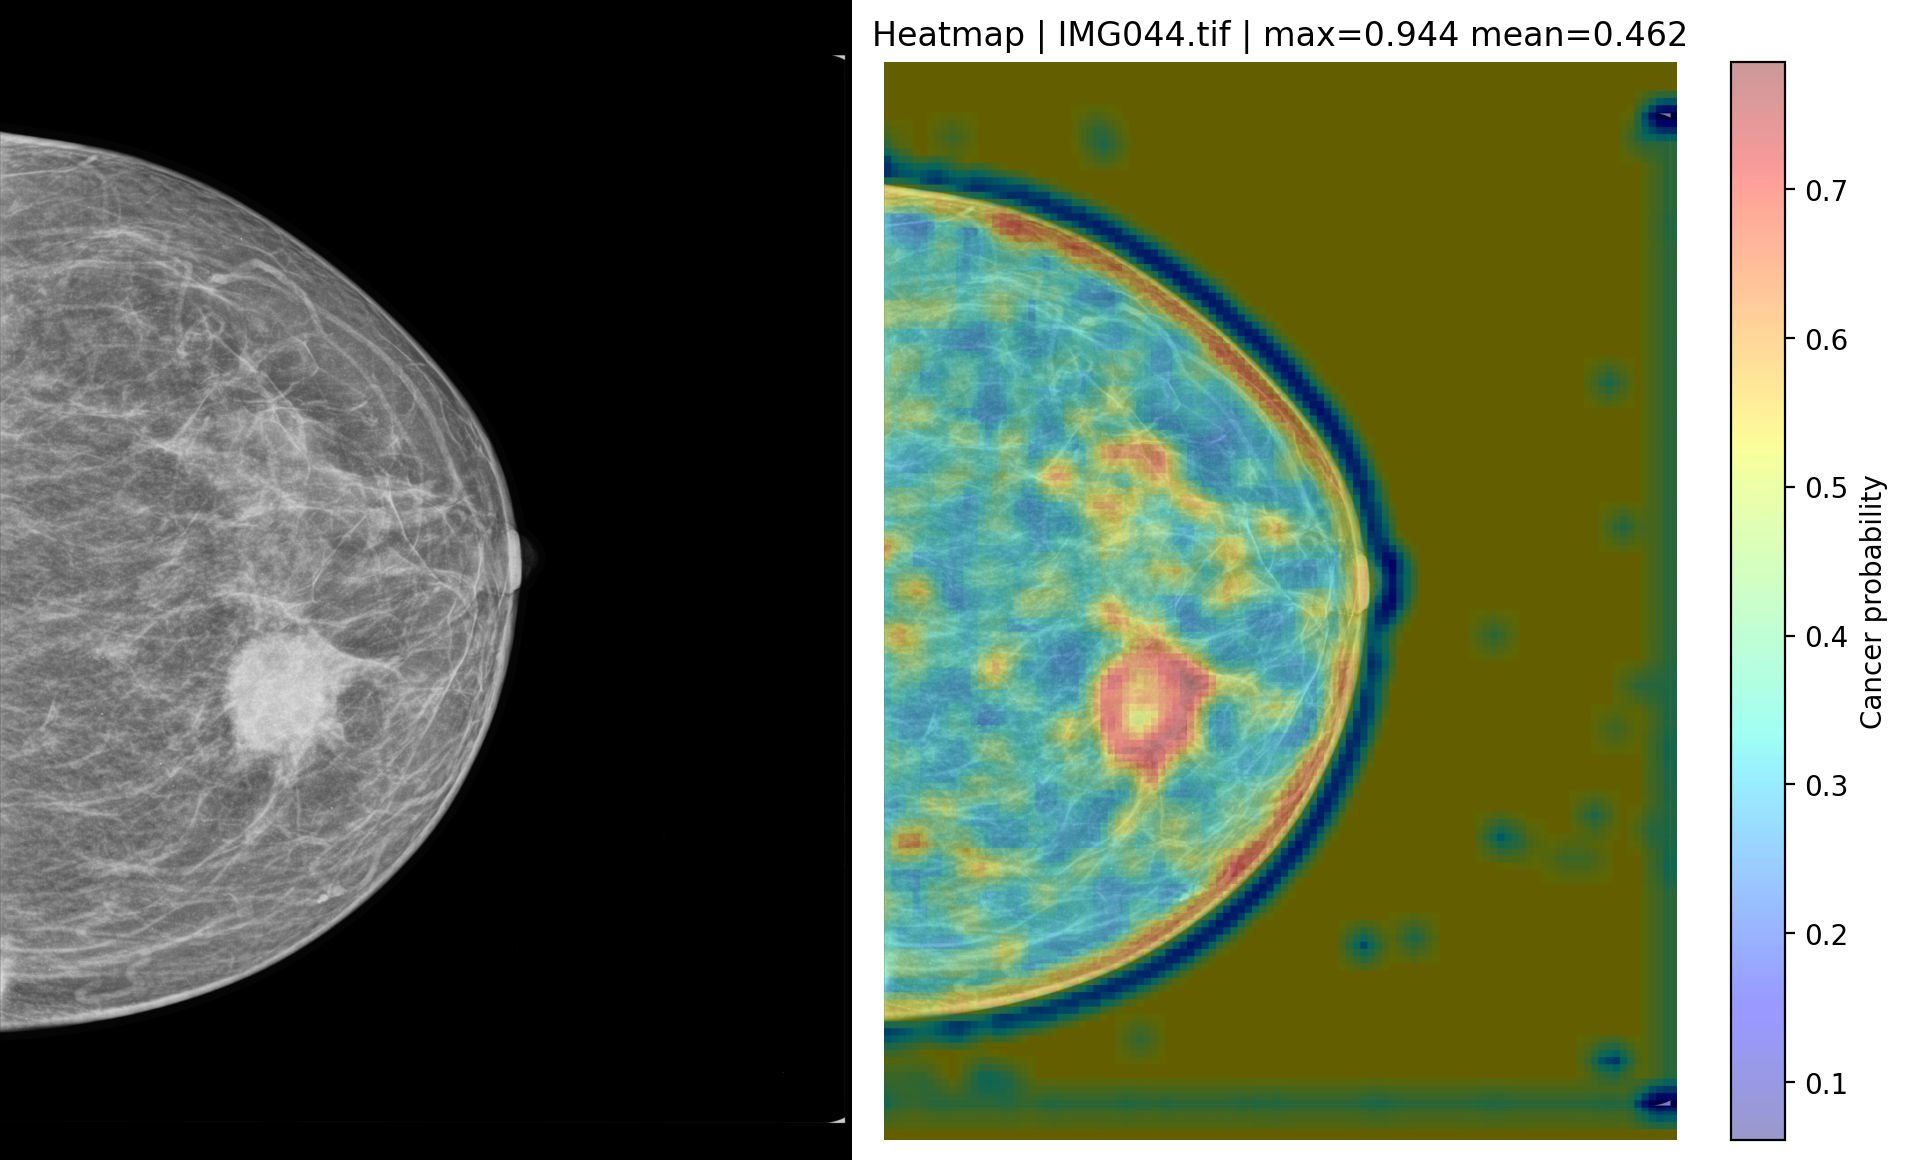
\includegraphics[width=0.49\textwidth]{../results/triangular_square_shape_sensitive/exp_008/heatmaps_pairs/IMG044_pair.png}
    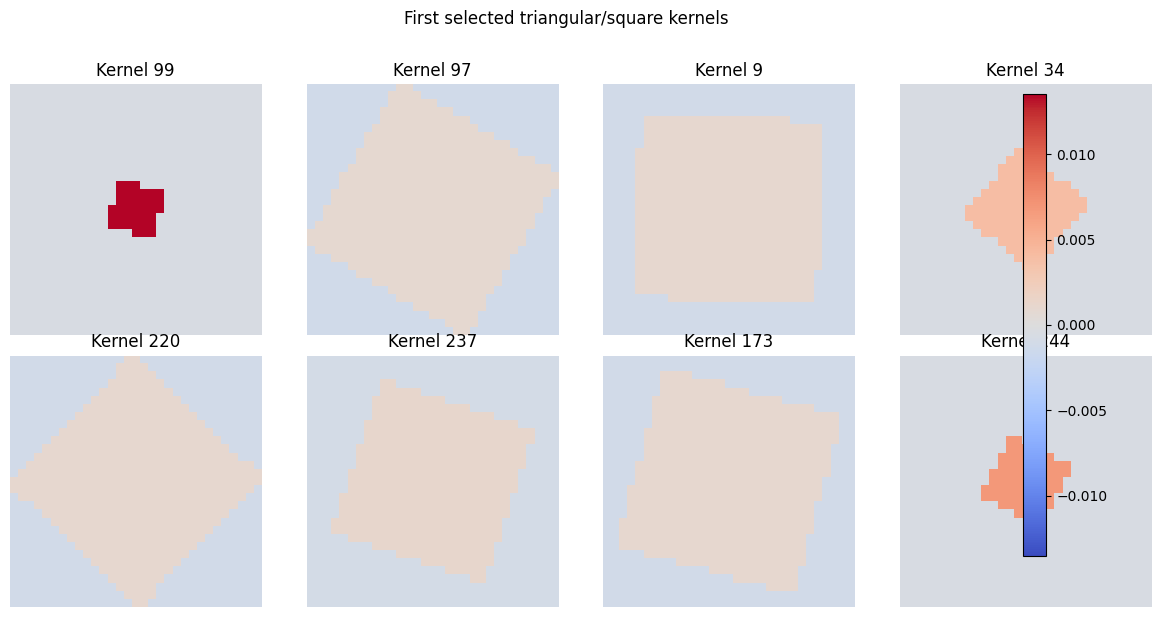
\includegraphics[width=0.49\textwidth]{../results/triangular_square_shape_sensitive/exp_008/kernels.png}
    \caption{Square kernel heatmap; It can be noticed that the middle of the cancerous area is not being highlighted.}
\end{figure}

\section*{Conclusion}

The main conclusion is that the circular radial prior is the most suitable of the tested kernel families for this task. It gives the highest test performance and the clearest localization, which suggests that the target structures are better matched by circularly symmetric filters than by non-circular geometric ones.

The spike in the learned radial profile should not be read as a fully new structure discovered from scratch. It is mainly inherited from the rotation-invariant circular seed, which already carried a stripe-like preference that became concentrated at particular radii and was then strengthened during training.

The non-circular geometric results remain useful as ablation studies. They show that different kernels can still reach reasonably good accuracy because many of them capture overlapping contrast and texture cues, but they also confirm that removing the circular prior reduces both classification quality and heatmap quality. In practice, the unconstrained radial model is the strongest option for maximum performance, while the constrained radial variants are the better choice when interpretability is more important.

\end{document}
